%%%% Paramétrage du TD %%%%
\def\xxactivite{Révisions \ifprof -- Corrigé \else \fi} % \normalsize \vspace{-.4cm}
\def\xxauteur{\textsl{Xavier Pessoles}}


\def\xxnumchapitre{Révision 1 \vspace{.2cm}}
\def\xxchapitre{\hspace{.12cm} Résolution des problèmes de statique -- Statique 3D}
\def\xxonglet{\textsf{Rév -- Stat}}
\def\xxactivite{\ifcolle Colle \else TD 02\fi }
\def\xxauteur{\textsl{Xavier Pessoles}}

\def\xxpied{%
Révision statique -- Résolution des problèmes de statique 3D\\
Fiche 1 -- \xxactivite%
}

\def\xxtitreexo{Quille pendulaire}
\def\xxsourceexo{\hspace{.2cm} \footnotesize{Concours Commun Mines Ponts 2014}}

\def\xxcompetences{%
\textsl{%
\textbf{Savoirs et compétences :}\\
\vspace{-.3cm}
\footnotesize
\begin{itemize}
\item \textit{Res1.C2.SF1} : Proposer une méthode permettant la détermination d’une inconnue de liaison.
\item \textit{Res1.C3.SF1} : Choisir une méthode pour déterminer la valeur des paramètres conduisant à des positions d'équilibre.
\item \textit{Res2.C18} : Principe fondamental de la statique.
\item \textit{Res2.C19} : Équilibre d’un solide, d’un ensemble de solides.
\item \textit{Res2.C20} : Théorème des actions réciproques.
\end{itemize}
\normalsize
}}

\def\xxauteur{\textsl{Xavier Pessoles}}


\def\xxfigures{
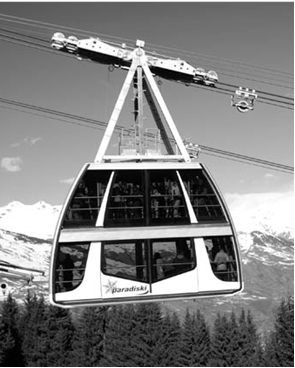
\includegraphics[width=.75\textwidth]{fig_00}
}%figues de la page de garde


\pagestyle{empty}


%%%%%%%% PAGE DE GARDE COURS
\ifcours
\begin{tikzpicture}[remember picture,overlay]
\node at (current page.north west)
{\begin{tikzpicture}[remember picture,overlay]
\node[anchor=north west,inner sep=0pt] at (0,0) {\includegraphics[width=\paperwidth]{\thechapterimage}};
\draw[anchor=west] (-2cm,-8cm) node [line width=2pt,rounded corners=15pt,draw=ocre,fill=white,fill opacity=0.6,inner sep=40pt]{\strut\makebox[22cm]{}};
\draw[anchor=west] (1cm,-8cm) node {\huge\sffamily\bfseries\color{black} %
\begin{minipage}{1cm}
\rotatebox{90}{\LARGE\sffamily\textsc{\color{ocre}\textbf{\xxnumpartie}}}
\end{minipage} \hfill
\begin{minipage}[c]{14cm}
\begin{titrepartie}
\begin{flushright}
\renewcommand{\baselinestretch}{1.1} 
\Large\sffamily\textsc{\textbf{\xxpartie}}
\renewcommand{\baselinestretch}{1} 
\end{flushright}
\end{titrepartie}
\end{minipage} \hfill
\begin{minipage}[c]{3.5cm}
{\large\sffamily\textsc{\textbf{\color{ocre} \discipline}}}
\end{minipage} 
 };
\end{tikzpicture}};
\end{tikzpicture}


\begin{tikzpicture}[overlay]
\node[shape=rectangle, 
      rounded corners = .25 cm,
	  draw= ocre,
	  line width=2pt, 
	  fill = ocre!10,
	  minimum width  = 2.5cm,
	  minimum height = 3cm,] at (18cm,0) {};
\node at (17.7cm,0) {\rotatebox{90}{\textbf{\Large\color{ocre}{\classe}}}};
%{};
\end{tikzpicture}

\vspace{3.5cm}

\begin{tikzpicture}[remember picture,overlay]
\draw[anchor=west] (-2cm,-6cm) node {\huge\sffamily\bfseries\color{black} %
\begin{minipage}{2cm}
\begin{center}
\LARGE\sffamily\textsc{\color{ocre}\textbf{\xxactivite}}
\end{center}
\end{minipage} \hfill
\begin{minipage}[c]{15cm}
\begin{titrechapitre}
\renewcommand{\baselinestretch}{1.1} 
\Large\sffamily\textsc{\textbf{\xxnumchapitre}}

\Large\sffamily\textsc{\textbf{\xxchapitre}}
\vspace{.5cm}

\renewcommand{\baselinestretch}{1} 
\normalsize\normalfont
\xxcompetences
\end{titrechapitre}
\end{minipage}  };
\end{tikzpicture}
\vfill

\begin{flushright}
\begin{minipage}[c]{.3\linewidth}
\begin{center}
\xxfigures
\end{center}
\end{minipage}\hfill
\begin{minipage}[c]{.6\linewidth}
\startcontents
\printcontents{}{1}{}
\end{minipage}
\end{flushright}

\begin{tikzpicture}[remember picture,overlay]
\draw[anchor=west] (4.5cm,-.7cm) node {
\begin{minipage}[c]{.2\linewidth}
\begin{flushright}

\includegraphics[width=2cm]{png/logoCC}
\end{flushright}
\end{minipage}
\begin{minipage}[c]{.2\linewidth}
\textsl{\xxauteur} \\
\textsl{\classe}
\end{minipage}
 };
\end{tikzpicture}
\newpage
\pagestyle{fancy}

\newpage
\pagestyle{fancy}

\else
\fi


%%%%%%%% PAGE DE GARDE TD
\iftd
%\begin{tikzpicture}[remember picture,overlay]
%\node at (current page.north west)
%{\begin{tikzpicture}[remember picture,overlay]
%\draw[anchor=west] (-2cm,-3.25cm) node [line width=2pt,rounded corners=15pt,draw=ocre,fill=white,fill opacity=0.6,inner sep=40pt]{\strut\makebox[22cm]{}};
%\draw[anchor=west] (1cm,-3.25cm) node {\huge\sffamily\bfseries\color{black} %
%\begin{minipage}{1cm}
%\rotatebox{90}{\LARGE\sffamily\textsc{\color{ocre}\textbf{\xxnumpartie}}}
%\end{minipage} \hfill
%\begin{minipage}[c]{13.5cm}
%\begin{titrepartie}
%\begin{flushright}
%\renewcommand{\baselinestretch}{1.1} 
%\Large\sffamily\textsc{\textbf{\xxpartie}}
%\renewcommand{\baselinestretch}{1} 
%\end{flushright}
%\end{titrepartie}
%\end{minipage} \hfill
%\begin{minipage}[c]{3.5cm}
%{\large\sffamily\textsc{\textbf{\color{ocre} \discipline}}}
%\end{minipage} 
% };
%\end{tikzpicture}};
%\end{tikzpicture}

%%%%%%%%%% PAGE DE GARDE TD %%%%%%%%%%%%%%%
%\begin{tikzpicture}[overlay]
%\node[shape=rectangle, 
%      rounded corners = .25 cm,
%	  draw= ocre,
%	  line width=2pt, 
%	  fill = ocre!10,
%	  minimum width  = 2.5cm,
%	  minimum height = 2.5cm,] at (18.5cm,0) {};
%\node at (17.7cm,0) {\rotatebox{90}{\textbf{\Large\color{ocre}{\classe}}}};
%%{};
%\end{tikzpicture}

% PARTIE ET CHAPITRE
%\begin{tikzpicture}[remember picture,overlay]
%\draw[anchor=west] (-1cm,-2.1cm) node {\large\sffamily\bfseries\color{black} %
%\begin{minipage}[c]{15cm}
%\begin{flushleft}
%\xxnumchapitre \\
%\xxchapitre
%\end{flushleft}
%\end{minipage}  };
%\end{tikzpicture}

% Bandeau titre exo
\begin{tikzpicture}[remember picture,overlay]
\draw[anchor=west] (-2cm,-6cm) node {\huge\sffamily\bfseries\color{black} %
\begin{minipage}{5cm}
\begin{center}
\LARGE\sffamily\color{ocre}\textbf{\textsc{\xxactivite}}

\begin{center}
\xxfigures
\end{center}

\end{center}
\end{minipage} \hfill
\begin{minipage}[c]{12cm}
\begin{titrechapitre}
\renewcommand{\baselinestretch}{1.1} 
\large\sffamily\textbf{\textsc{\xxtitreexo}}

\small\sffamily{\textbf{\textit{\color{black!70}\xxsourceexo}}}
\vspace{.5cm}

\renewcommand{\baselinestretch}{1} 
\normalsize\normalfont
\xxcompetences
\end{titrechapitre}
\end{minipage}  };
\end{tikzpicture}

\else
\fi


%%%%%%%% PAGE DE GARDE FICHE
\iffiche
\begin{tikzpicture}[remember picture,overlay]
\node at (current page.north west)
{\begin{tikzpicture}[remember picture,overlay]
\draw[anchor=west] (-2cm,-3.25cm) node [line width=2pt,rounded corners=15pt,draw=ocre,fill=white,fill opacity=0.6,inner sep=40pt]{\strut\makebox[22cm]{}};
\draw[anchor=west] (1cm,-3.25cm) node {\huge\sffamily\bfseries\color{black} %
\begin{minipage}{1cm}
\rotatebox{90}{\LARGE\sffamily\textsc{\color{ocre}\textbf{\xxnumpartie}}}
\end{minipage} \hfill
\begin{minipage}[c]{14cm}
\begin{titrepartie}
\begin{flushright}
\renewcommand{\baselinestretch}{1.1} 
\large\sffamily\textsc{\textbf{\xxpartie} \\} 

\vspace{.2cm}

\normalsize\sffamily\textsc{\textbf{\xxnumchapitre -- \xxchapitre}}
\renewcommand{\baselinestretch}{1} 
\end{flushright}
\end{titrepartie}
\end{minipage} \hfill
\begin{minipage}[c]{3.5cm}
{\large\sffamily\textsc{\textbf{\color{ocre} \discipline}}}
\end{minipage} 
 };
\end{tikzpicture}};
\end{tikzpicture}


\begin{tikzpicture}[overlay]
\node[shape=rectangle, 
      rounded corners = .25 cm,
	  draw= ocre,
	  line width=2pt, 
	  fill = ocre!10,
	  minimum width  = 2.5cm,
%	  minimum height = 2.5cm,] at (18.5cm,0.5cm) {};
	  minimum height = 2.5cm,] at (18.5cm,0cm) {};
\node at (17.7cm,0) {\rotatebox{90}{\textsf{\textbf{\large\color{ocre}{\classe}}}}};
%{};
\end{tikzpicture}



\else
\fi




\setlength{\columnseprule}{.1pt}

\pagestyle{fancy}
\thispagestyle{plain}

\vspace{5cm}

\def\columnseprulecolor{\color{ocre}}
\setlength{\columnseprule}{0.4pt} 

\setcounter{exo}{0}

%%%%%%%%%%%%%%%%%%%%%%%%%%%%%%%%%%%%%%%%%%%%%%%%%%
\ifprof
%\begin{multicols}{2}
\else
\begin{multicols}{2}
\fi

\section*{Mise en situation}
\ifprof
\else

Les actions de l'air et de l'eau permettent au voilier d'avancer mais provoquent aussi son inclinaison autour de l'axe longitudinal $\vect{z_N}$. C’est le phénomène de gîte. Pour contrebalancer ce mouvement et éviter que le voilier ne se couche sur l’eau, la quille joue le rôle de contrepoids. 


\begin{center}
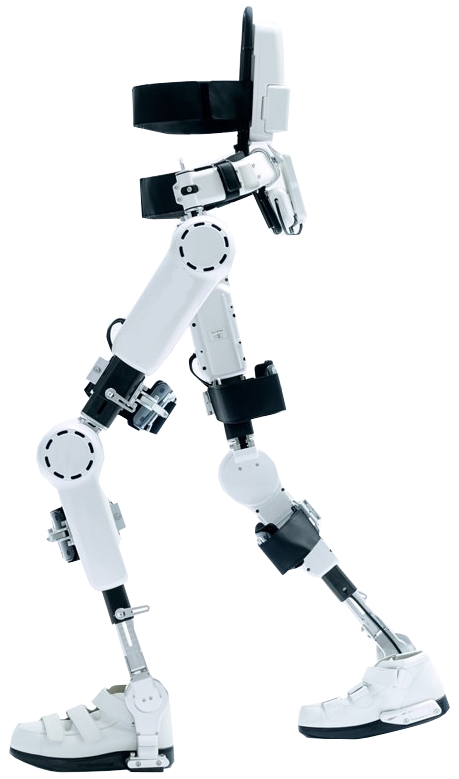
\includegraphics[width=.8\linewidth]{fig_01}
%\textit{}
\end{center}

Une évolution récente des voiliers de course océanique a été de les doter d’une quille pendulaire. Cette quille est en liaison pivot d’axe $\left(O,\vect{z_N} \right)$ avec la coque du navire et peut être orientée d’un côté ou de l’autre du navire. Une fois l’orientation désirée obtenue, tout mouvement dans la liaison pivot est supprimé par le blocage en rotation de celle-ci. 
%Cette quille est généralement constituée d’un voile immergé dans l’eau à l’extrémité duquel se trouve un lest profilé. L’efficacité de la quille dépend de la masse du lest et de la longueur du voile. Ces deux paramètres présentent des limitations : le lest ne peut être trop important sous peine de solliciter dangereusement le voile de quille et la longueur de quille est limitée par le tirant d’eau maximal admissible (il faut permettre l’entrée dans les ports sans toucher le fond !).


\begin{center}
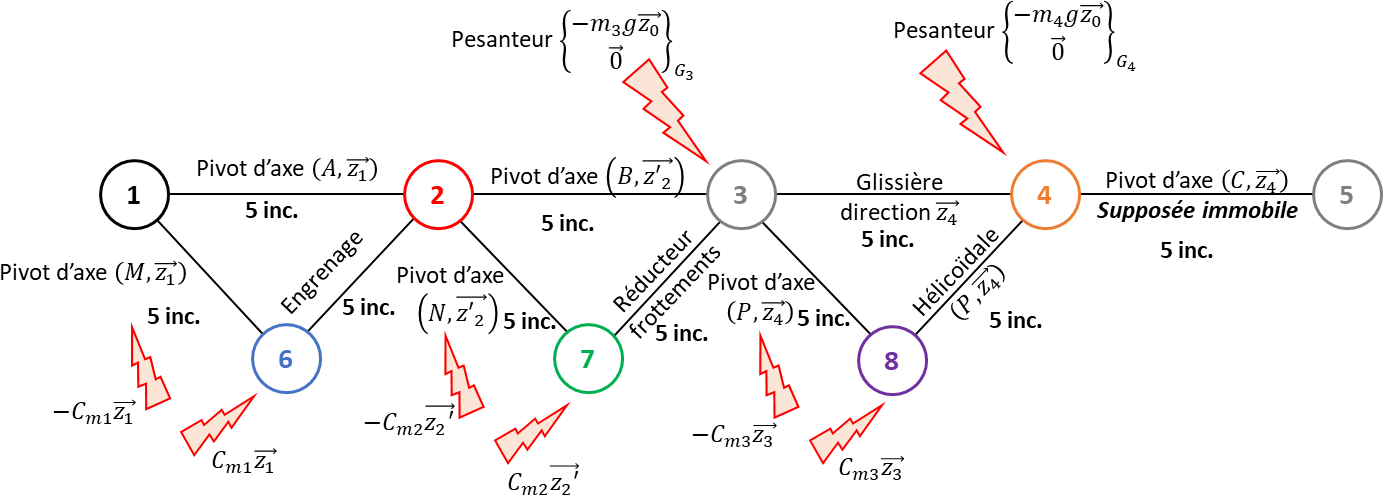
\includegraphics[width=.8\linewidth]{fig_02}
%\textit{}
\end{center}
\fi
\begin{obj}
L’objectif de cette partie est de valider la solution technologique de réalisation de la liaison pivot  entre la quille et la coque.
\end{obj}

\ifprof
\else

\begin{center}
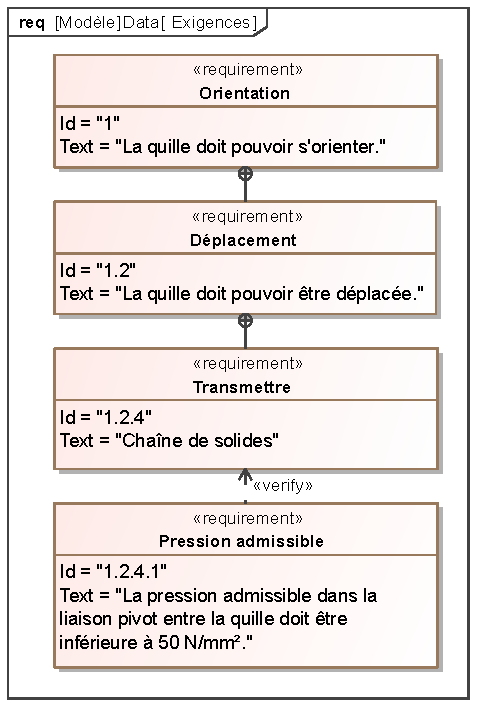
\includegraphics[width=.8\linewidth]{Exigences}
%\textit{}
\end{center}
\fi
\subsection*{Travail à réaliser}
\ifprof
\else

Le modèle de calcul est donné dans les figures suivantes.

\textbf{Hypothèses}

\begin{itemize}
\item Les liaisons sont toutes parfaites.
\item \textbf{Seul le vérin 2--4 est moteur} ($F_{h3}=0$ -- les solides 3 et 5 ne sont donc pas à prendre en compte). Le fluide (pression hydraulique) agit simultanément sur les pièces 2 et 4. L’action du fluide sur 2 est donnée par 
$\torseurstat{T}{\text{ph}}{2}=\torseurl{F_{h2}\vect{x_2}}{\vect{0}}{C}$.
\item Les actions mécaniques de frottement visqueux provenant du déplacement du fluide dans les canalisations sont toutes négligées.% ($k=0$).
\item Les actions hydrodynamiques sur le voile et le lest de quille sont également négligées.
\item Les poids des éléments constitutifs des deux vérins sont négligés.
\item On note $G_1$ le centre d'inertie de la quille 1 et $M_1$ la masse de la quille.
%\item La variation de $\theta_2$ pour toute l’amplitude du mouvement de relevage de la quille est faible; $\theta_2$ sera pris égal à 0 : les bases $\mathcal{B}_2$, $\mathcal{B}_4$ et $\mathcal{B}_N$ sont donc confondues. Cependant l’angle $\theta_1$ est différent de zéro.
\item Les bases $\mathcal{B}_2$ et $\mathcal{B}_N$ sont considérées confondues. Cependant l’angle $\theta_1$ est différent de zéro.
\item Les conditions de déplacement rendent négligeables les effets dynamiques. Les théorèmes de la statique seront donc utilisés dans la suite.
\end{itemize}

\begin{center}
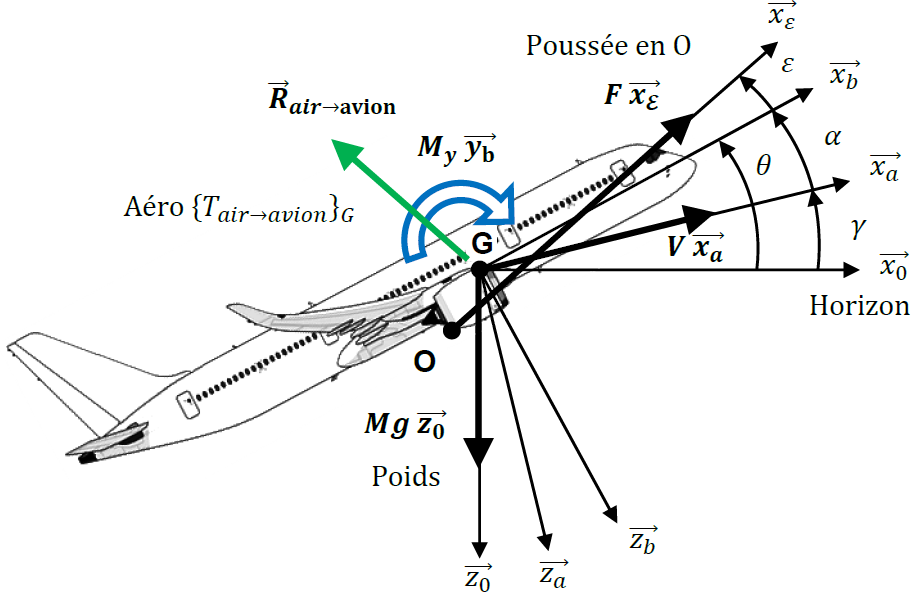
\includegraphics[width=.7\linewidth]{fig_03}

\textit{Modèle volumique 3D}
\end{center}

\begin{center}
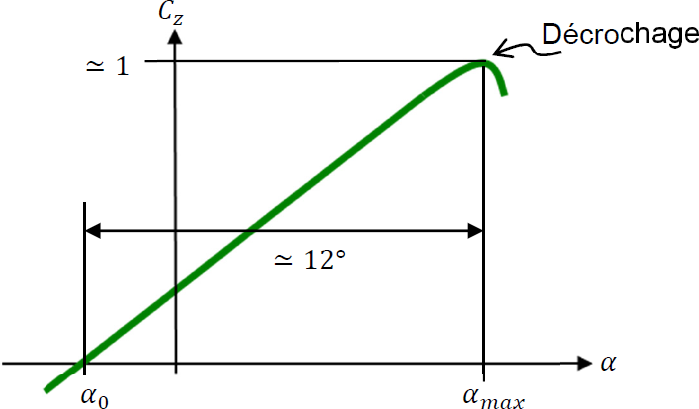
\includegraphics[width=\linewidth]{fig_04}

%\vspace{-.2cm}

$\vect{OA}=R\vect{y_1}$, 
$\theta_1 =\angl{x_N}{x_1}$,
$\vect{OG_1}=-L_1\vect{y_1}$,
$\vect{AA_2}=-d\vect{z_N}$
$\vect{AA_3}=d\vect{z_N} $.

%\vspace{-.8cm}

\textit{Schéma cinématique 3D}
\end{center}
\fi
\subparagraph{}\textit{
En isolant le bon système, montrer que l’action de 2 sur 1 en $A_2$ est représentable par le glisseur dont la forme sera notée : $\torseurl{F_{21}\vect{x}_2}{\vect{0}}{A_2}$ ou 
$\torseurl{F_{21}\vect{x}_N}{\vect{0}}{A_2}$ puisque $\mathcal{B}_N=\mathcal{B}_2$.}
\ifprof
\begin{corrige}
\begin{multicols}{2}
Le graphe de structure associé au modèle cinématique est donné dans la figure suivante. 
\begin{center}
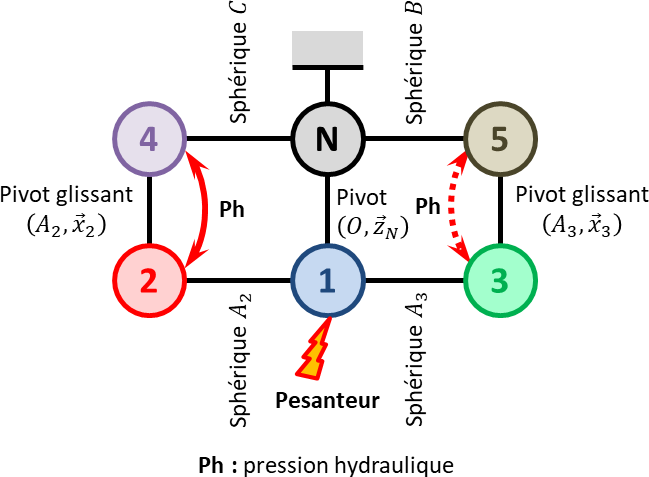
\includegraphics[width=\linewidth]{cor_01}
%\textit{Modèle volumique 3D}
\end{center}

On isole l'ensemble \textbf{\{4+2\}}. Cet ensemble est soumis à 2 glisseurs. D'après le PFS les deux actions mécaniques ont donc même direction (la droite $(A_2C)$, vecteur $\vect{x}_2=\vect{x}_N$), la même norme ($\left|F_{21} \right|$)et le sens opposé. On a donc : $\torseurstat{T}{0}{4}+\torseurstat{T}{1}{2}=\{0\} \Leftrightarrow \torseurstat{T}{0}{4}=\torseurstat{T}{2}{1}$ et donc  $\torseurstat{T}{2}{1}=\torseurl{F_{21}\vect{x}_N}{\vect{0}}{A_2}$.
\end{multicols}
\end{corrige}
\else
\fi

\subparagraph{}\textit{
Déterminer l'effort $F_{21}$ nécessaire au déplacement de la quille.}
\ifprof
\begin{corrige}
On isole la quille 1. 

On réalise le BAME : 
\begin{itemize}
\item action de 2 sur 1 : $\torseurstat{T}{2}{1}=\torseurl{F_{21}\vect{x_N}}{\vect{0}}{A_2}$;
\item action de 3 sur 1 : $\torseurstat{T}{3}{1}=\{0\}$ (pas d'action mécanique dans le vérin);
\item action de N sur 1 : $\torseurstat{T}{N}{1}_{\text{pivot}}=\torseurl{X_{N1p}\vect{x_N}+Y_{N1p}\vect{y_N}+Z_{N1p}\vect{z_N}}{L_{N1p}\vect{x_N}+M_{N1p}\vect{y_N}}{O}$;
\item action de la pesanteur sur 1 : $\torseurstat{T}{\text{pes}}{1}=\torseurl{-M_1g\vect{y_N}}{\vect{0}}{G_1}$.
\end{itemize}

La quille étant en pivot d'axe $\axe{O}{z_N}$ par rapport à \textbf{0}, réalisons le théorème du moment statique en $O$ en projection sur $\vect{z_N}$ :

\noindent
$\left(\vect{OA_2}\wedge F_{21}\vect{x_N}  + 
\vect{OG_1}\wedge -M_1g\vect{y_N} \right) \vect{z_N} = {0}$ 

\noindent
$\Leftrightarrow  \left(\left( R\vect{y_1} - d\vect{z_N}\right)\wedge F_{21}\vect{x_N}  
+L_1\vect{y_1}\wedge M_1g\vect{y_N} \right) \vect{z_N} = {0}$

\noindent
$\Leftrightarrow 
-F_{21}\vect{y_N}\left( R\vect{y_1} - d\vect{z_N}\right)  
+L_1 M_1g\left(\vect{x_N} \cdot \vect{y_1}\right) = {0}$
\noindent

\noindent
$\Leftrightarrow 
-RF_{21}\cos \theta_1
-L_1 M_1g\sin\theta_1 = {0}$

\noindent
$\Leftrightarrow F_{21}=-\dfrac{L_1}{R} M_1g\tan\theta_1 $.

\end{corrige}
\else
\fi

\subparagraph{}\textit{Exprimer, en fonction de $d$, $g$,
$M_1$, et $F_{21}$, par ses éléments de réduction en $O$, dans la base $\left( \vect{x_N} , \vect{y_N} , \vect{z_N} \right)$, le torseur d’action mécanique de $N$
sur 1, $\torseurstat{T}{N}{1}_{\text{pivot}}$.}
\ifprof
\begin{corrige} ~\\

\begin{center}
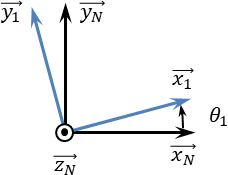
\includegraphics[width=.25\linewidth]{cor_02}
%\textit{Modèle volumique 3D}
\end{center}


En conservant le même isolement et le même bilan des actions mécaniques, on réalise le PFS en $O$ et on a : 
$$
\left\{
\begin{array}{l}
F_21\vect{x_N}+X_{N1p}\vect{x_N}+Y_{N1p}\vect{y_N}+Z_{N1p}\vect{z_N} - M_1g\vect{y_N} = \vect{0}\\
\vect{OA_2}\wedge F_{21}\vect{x_N}  + 
\vect{OG_1}\wedge -M_1g\vect{y_N}  +L_{N1p}\vect{x_N}+M_{N1p}\vect{y_N}= \vect{0} \\
\end{array}
\right.
$$



$$ \Leftrightarrow
\left\{
\begin{array}{l}
F_{21}\vect{x_N}+X_{N1p}\vect{x_N}+Y_{N1p}\vect{y_N}+Z_{N1p}\vect{z_N} - M_1g\vect{y_N} = \vect{0}\\
 F_{21}\left( R\vect{y_1} \wedge \vect{x_N}- d\vect{z_N}\wedge \vect{x_N}\right)  
-L_1M_1g \sin \theta \vect{z_N} +L_{N1p}\vect{x_N}+M_{N1p}\vect{y_N} = \vect{0} \\
\end{array}
\right.
$$

$$ \Leftrightarrow
\left\{
\begin{array}{l}
F_{21}\vect{x_N}+X_{N1p}\vect{x_N}+Y_{N1p}\vect{y_N}+Z_{N1p}\vect{z_N} - M_1g\vect{y_N} = \vect{0}\\
 F_{21}\left( - R\cos\theta_1\vect{z_N}- d\vect{y_N}\right)  
-L_1M_1g \sin \theta \vect{z_N} +L_{N1p}\vect{x_N}+M_{N1p}\vect{y_N} = \vect{0} \\
\end{array}
\right.
$$

On a : 
$$
\left\{
\begin{array}{l}
F_{21}+X_{N1p} = 0 \\
Y_{N1p}- M_1g = 0 \\
Z_{N1p}=0 \\
\end{array}
\right.
\quad
\left\{
\begin{array}{l}
 L_{N1p} = {0} \\
- dF_{21}+M_{N1p} = {0} \\
-F_{21}  R\cos\theta_1-L_1M_1g \sin \theta  = {0} \\
\end{array}
\right.
$$

$$
\Leftrightarrow
\left\{
\begin{array}{l}
X_{N1p} = - F_{21}\\
Y_{N1p}= M_1g  \\
Z_{N1p}=0 \\
\end{array}
\right.
\quad
\left\{
\begin{array}{l}
 L_{N1p} = {0} \\
M_{N1p} =dF_{21} \\
0 = 0\\
\end{array}
\right.
$$



\end{corrige}
\else
\fi

\ifprof
\else

La liaison pivot de $N$ sur $1$ est composée de deux paliers modélisés par une liaison sphère-cylindre et une liaison sphérique placées en parallèle (voir figure suivante). La
géométrie de l’assemblage est telle que :
$\vect{OO_2}= e\vect{z_N}$ ; $\vect{OO_1}= -e\vect{z_N}$ avec $e=\SI{350}{mm}$.




\begin{center}
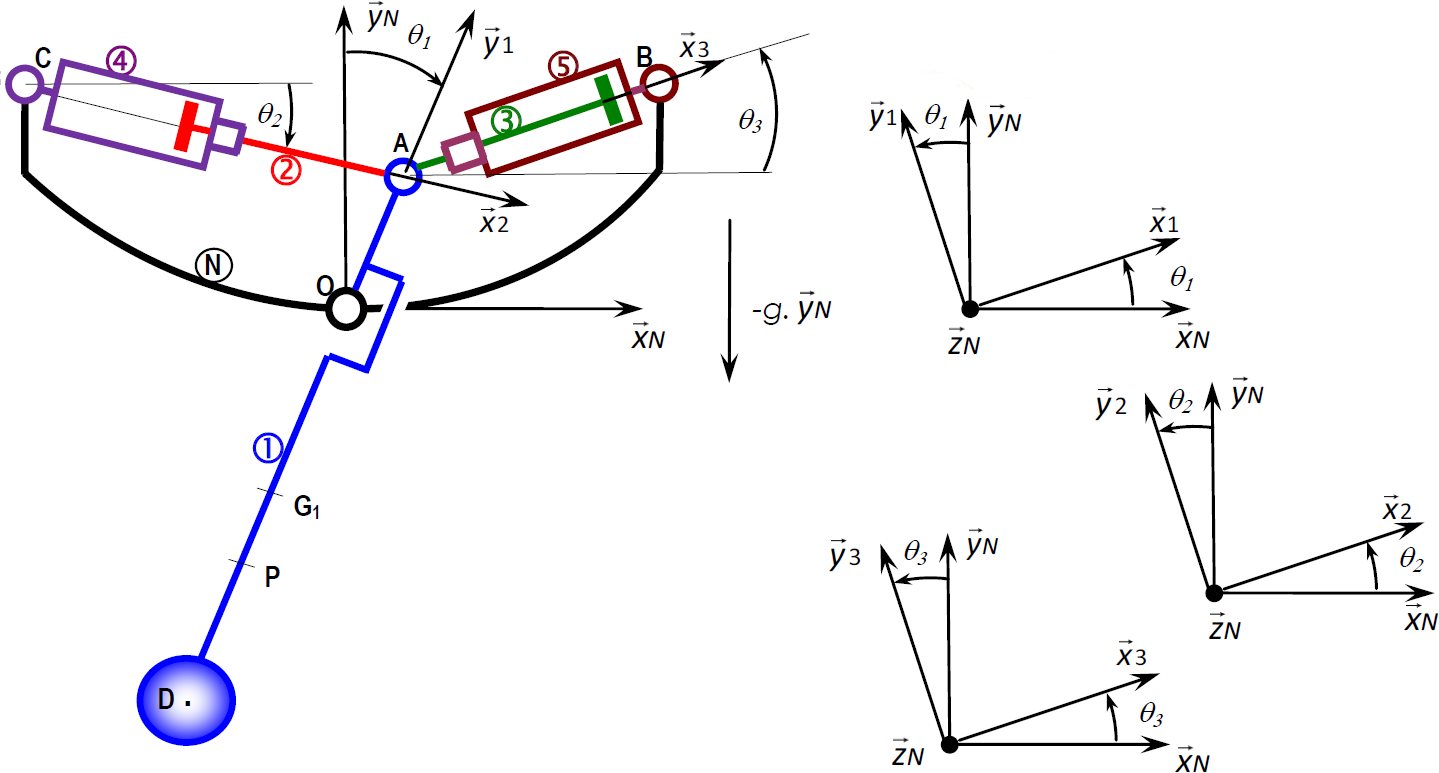
\includegraphics[width=.8\linewidth]{fig_05}
%\textit{Modèle volumique 3D}
\end{center}
\fi

\subparagraph{}\textit{Écrire la relation liant les torseurs d’action mécanique $\torseurstat{T}{N}{1}_{\text{sphère-cylindre}}$, $\torseurstat{T}{N}{1}_{\text{sphérique}}$ et $\torseurstat{T}{N}{1}_{\text{pivot}}$.
En déduire, par ses éléments de réduction en $O_1$, dans la
base $\mathcal{B}_N=\left(\vect{x_N} , \vect{y_N} , \vect{z_N} \right)$, en fonction de $d$, $g$, $M_1$, et $F_{21}$, le torseur d’action mécanique de $N$ sur 1 en $O_1$, $\torseurstat{T}{N}{1}_{\text{sphère-cylindre}}$.}
\ifprof
\begin{corrige} ~\\
On a $\torseurstat{T}{N}{1}_{\text{sphère-cylindre}} + \torseurstat{T}{N}{1}_{\text{sphérique}} = \torseurstat{T}{N}{1}_{\text{pivot}}$. 

En conséquences :
$\torseurstat{T}{N}{1}_{\text{sphère-cylindre}}
= \torseurl{X_{N1sc}\vect{x_N}+Y_{N1sc}\vect{y_N}}{\vect{0}}{O_1}
= \torseurl{X_{N1sc}\vect{x_N}+Y_{N1sc}\vect{y_N}}{-e X_{N1sc} \vect{y_N}+eY_{N1sc} \vect{x_N}}{O}$

et 
$\torseurstat{T}{N}{1}_{\text{sphérique}}
= \torseurl{X_{N1s}\vect{x_N}+Y_{N1s}\vect{y_N}+Z_{N1s}\vect{z_N}}{\vect{0}}{O_2}
= \torseurl{X_{N1s}\vect{x_N}+Y_{N1s}\vect{y_N}+Z_{N1s}\vect{z_N}}{e X_{N1s} \vect{y_N}-eY_{N1s} \vect{x_N}}{O}$.

Au final, on a :
$$
\left\{
\begin{array}{l}
X_{N1p} = X_{N1sc}+X_{N1s} \\
Y_{N1p}= Y_{N1sc}+Y_{N1s} \\
Z_{N1p}= Z_{N1s}  \\
\end{array}
\right.
\text{et }
\left\{
\begin{array}{l}
L_{N1p} =e Y_{N1sc}-e Y_{N1s} \\
M_{N1p}= -e X_{N1sc}-e Y_{N1s} \\
0 = 0\\
\end{array}
\right. .
$$

$$
\left\{
\begin{array}{l}
X_{N1p} = X_{N1sc}+X_{N1s} \\
Y_{N1p}= Y_{N1sc}+Y_{N1s} \\
Z_{N1p}= Z_{N1s}  \\
\end{array}
\right.
\text{et }
\left\{
\begin{array}{l}
L_{N1p} =e Y_{N1sc}-e Y_{N1s} \\
M_{N1p}= -e X_{N1sc}-e Y_{N1s} \\
\end{array}
\right. 
\Rightarrow 
\left\{
\begin{array}{l}
- F_{21} = X_{N1sc}+X_{N1s} \\
M_1g= Y_{N1sc}+Y_{N1s} \\
0= Z_{N1s}  \\
\end{array}
\right.
\text{et }
\left\{
\begin{array}{l}
0 =e Y_{N1sc}-e Y_{N1s} \\
dF_{21}= -e X_{N1sc}-e Y_{N1s} \\
\end{array}
\right. 
$$

$$
\Rightarrow 
\left\{
\begin{array}{l}
- F_{21} = X_{N1sc}+X_{N1s} \\
M_1g= 2Y_{N1sc} \\
Z_{N1s} = 0  \\
\end{array}
\right.
\text{et }
\left\{
\begin{array}{l}
 Y_{N1sc}= Y_{N1s} \\
dF_{21}= -e X_{N1sc}-e Y_{N1sc} \\
\end{array}
\right.
\Rightarrow 
%\left\{
%\begin{array}{l}
%- F_{21} = X_{N1sc}+X_{N1s} \\
%Y_{N1sc} = \dfrac{M_1g}{2}\\
%Z_{N1s} = 0  \\
%\end{array}
%\right.
%\text{et }
\left\{
\begin{array}{l}
X_{N1sc}=-\dfrac{d}{e}F_{21} - \dfrac{M_1g}{2} \\
Y_{N1sc} = \dfrac{M_1g}{2}\\% Y_{N1sc}= Y_{N1s} \\
\end{array}
\right. .
$$

%$\Leftrightarrow F_{21}=\dfrac{L_1}{R} M_1g\tan\theta_1 $.
\end{corrige}
\else
\fi



\subsection*{Retour sur le cahier des charges}
\ifprof
\else

On se place dans les conditions suivantes :
\begin{itemize}
\item la valeur maximale de l’action $F_{21}$ a été estimée dans l’étude précédente : $F_{21\text{Maxi}}=\SI{2e5}{N}$. De
plus : $M_1 g = \SI{4,1e4}{N}$, $e=\SI{350}{mm}$ et $d=\SI{200}{mm}$;
\item les << paliers >> sont constitués côté quille de contacts cylindriques de diamètre $d_c =\SI{80}{mm}$ et de longueur $L_c =\SI{50}{mm}$, $O_1$ étant dans le plan médian du cylindre de contact. Un coussinet de nylon
sert d’interface entre la quille et le navire. Ce coussinet est caractérisé par sa pression de contact
maximale admissible : $p_{\text{adm}}= \SI{50}{N.mm^{-2}}$. Par ailleurs on peut montrer que lorsqu'un coussinet est chargé par une pression uniforme sur un demi-cylindre, la relation entre l'effort radial est la pression est donnée par : $p_{21}=\dfrac{F}{d_cL_c}$.
\end{itemize}
\fi

\subparagraph{}\textit{Dans ces conditions, calculer la valeur de l’effort radial (perpendiculaire à l’axe géométrique du coussinet) qui sollicite ce coussinet en $O_1$.
Valider ensuite l’usage de ce coussinet de nylon.}
\ifprof
\begin{corrige}
On a 
$F = \sqrt{X_{N1sc}^2+Y_{N1sc}^2}
= \sqrt{\left(-\dfrac{d}{e}F_{21} - \dfrac{M_1g}{2} \right)^2+\left( \dfrac{M_1g}{2}\right)^2}$

$= \sqrt{\left(-\dfrac{200}{350}200000 -  \dfrac{41000}{2}\right)^2+\left( \dfrac{41000}{2}\right)^2}$
$=\SI{136336}{N}$.
% \sqrt{\left(-114285,7 -  20500\right)^2+\left( 20500\right)^2}$

Et donc, $p_{21}=\dfrac{136336}{80\cdot 50}\simeq \SI{34}{MPa}<p_{\text{adm}}$.
\end{corrige}
\else
\fi

\ifcolle
\else
\ifprof
\else
\subsubsection*{Corrigé résumé}
\footnotesize
\begin{enumerate}
\item .
\item $\Leftrightarrow F_{21}=-\dfrac{L_1}{R} M_1g\tan\theta_1 $.
\item $X_{N1p} = - F_{21}$, $Y_{N1p}= M_1g$, $Z_{N1p}=0$, $
 L_{N1p} = {0}$, $M_{N1p} =dF_{21}$.
\item $X_{N1sc}=-\dfrac{d}{e}F_{21} - \dfrac{M_1g}{2}$ et $Y_{N1sc} = \dfrac{M_1g}{2}$ (ou $X_{N1sc}=-\dfrac{e+d}{2e}F_{21}$).
\item $F=\SI{136336}{N}$ et $p_{21}\simeq \SI{34}{MPa}<p_{\text{adm}}$ (ou $F=\SI{158000}{N}$ et $p_{21}\simeq \SI{40}{MPa}$).
\end{enumerate}
\normalsize
\fi
\fi
%\ifprof
%\else


\ifprof
\else
\end{multicols}
\fi




